
%%%  یک نمونه پروپوزال کارشناسی ارشد، نسخه 0.4
%%%  وحید دامن‌افشان، دانشگاه تبریز،       http://www.damanafshan.ir
%%%   آپدیت شده در تیرماه ۹۱
%توضیحات مربوط به هر بسته یا دستور را می‌توانید در خط بالای آن ببینید.
%-----------------------------------
%%% شخصی‌سازی توسط نوید خزاعی (نخ) در اردیبهشت‌ماه ۹۳ - پروپوزال کارشناسی ارشد
\documentclass[12pt,a4paper]{article}
%در ورژن جدید زی‌پرشین برای تایپ متن‌های ریاضی، این سه بسته، حتماً باید فراخوانی شود
\usepackage{amsthm,amssymb,amsmath}
%دستوری برای وارد کردن واژه‌نامه انگلیسی به فارسی
\newcommand\persiangloss[2]{#1\dotfill\lr{#2}\\}
%%% ------- اضافه شده توسط نخ ------
%%% دستوری برای پنهان کردن چیزی از فهرست
\newcommand{\nocontentsline}[3]{}
\newcommand{\tocless}[2]{\bgroup\let\addcontentsline=\nocontentsline#1{#2}\egroup}
\usepackage[bottom]{footmisc}
\usepackage{indentfirst}
%\usepackage[english]{babel}
%\usepackage{caption}
%\captionsetup[figure]{name=شکل}

%\captionsetup[contentsname]{name=فهرست}
%\renewcommand{\contentsname}{فهرست مطالب}

% ------ پایان تغییرات نخ
%بسته‌ای برای تنطیم حاشیه‌های بالا، پایین، چپ و راست صفحه
%\usepackage[top=50mm, bottom=50mm, left=50mm, right=50mm]{geometry}
%بسته‌ای برای نمایش تصاویر قرار داده شده در متن
\usepackage{graphicx}
\usepackage{subcaption}
% بسته‌ و دستوراتی برای ایجاد لینک‌های رنگی با امکان جهش
\usepackage[pagebackref=false,colorlinks,linkcolor=blue,citecolor=magenta]{hyperref}
% چنانچه قصد پرینت گرفتن نوشته خود را دارید، خط بالا را غیرفعال و  از دستور زیر استفاده کنید چون در صورت استفاده از دستور زیر‌‌، 
% لینک‌ها به رنگ سیاه ظاهر خواهند شد و برای پرینت گرفتن، مناسب‌تر خواهد بود.
%\usepackage[pagebackref=false]{hyperref}
%بسته‌ای برای ظاهر شدن «مراجع»  در فهرست مطالب
\usepackage{tocbibind}
%فراخوانی بسته زی‌پرشین و دستورات مربوط به نوع فونت‌ها
\usepackage{xepersian}
\settextfont[Scale=1.1]{B Nazanin}
\DefaultMathsDigits


% وارد کردن دستور بالا الزامی نیست؛ چون در صورت وارد نکردن آن، فونت پیش‌فرض به صورت خودکار، فراخوانی می‌شود.
% چنانچه می‌خواهید که اعداد داخل فرمول‌ها، فارسی باشد، دستور زیر را فعال کنید
%\setdigitfont{Yas}
%%%%%%%%%%%%%%%%%%%%%%%%%%%%%%%%%%%%%%%%%%%%%%%%%%%
% تعریف قلم‌های فارسی و انگلیسی برای استفاده در بعضی از قسمت‌های متن
\defpersianfont\titr[Scale=1]{B Titr}
\defpersianfont\nastaliq[Scale=1.5]{IranNastaliq}
\defpersianfont\traffic[Scale=1]{B Traffic}
\defpersianfont\yekan[Scale=1]{B Yekan}
%اگر فونت‌های بالا را ندارید، دو خط بالا را غیر فعال و دو خط زیر را فعال کنید
%\defpersianfont\traffic[Scale=1]{XB Roya}
%\defpersianfont\yekan[Scale=1]{XB Kayhan}
%%%%%%%%%%%%%%%%%%%%%%%%%%%%%%%%%%%%%%%%%%%%%%%%%%%
% تعریف و نحوه ظاهر شدن قضایا، لم‌ها، تعریف‌ها و ...
\theoremstyle{definition}
\newtheorem{definition}{تعریف}[section]
\theoremstyle{theorem}
\newtheorem{theorem}[definition]{قضیه}
\newtheorem{lemma}[definition]{لم}
\newtheorem{proposition}[definition]{گزاره}
\newtheorem{corollary}[definition]{نتیجه}
\newtheorem{remark}[definition]{ملاحظه}
\theoremstyle{definition}
\newtheorem{example}[definition]{مثال}
%%%%%%%%%%%%%%%%%%%%%%%%%%%%%%%%%%%%%%%%%%%%%%%%%%%
\begin{document}
% دستوری جهت حذف کردن شماره صفحه و سربرگ، در صورت وجود (فقط در صفحه جاری)
\thispagestyle{empty}
\vspace*{-28mm}
% نحوه درج کردن لوگوی دانشگاه
\centerline{
\includegraphics[height=5cm]{logo.png}}
\begin{center}
%دستوری برای کم کردن فاصله بین لوگو و خط پایین آن
\vspace{-6mm}

گروه مستقل مهندسی رباتیک
%دستوری برای تعیین فاصله بین دو خط
\\[1.5cm]

{\large
\textbf { 
پیشنهاد موضوع تحقیقاتی برای رساله‌ی کارشناسی ارشد
}
\\[1.2cm]
عنوان فارسی:
\\[.4cm]
}
%دستوری برای تعیین فاصله بین خطوط (نه دو خط) و تا وقتی که مقدار آن تغییر نکند، فاصله بین خطوط، همین مقدار است.
\baselineskip=1cm
{\Large \titr
تشخیص و مکان‌یابی بی‌درنگ تابلوهای راهنما و متن فارسی در ویدیوهای ترافیکی شهری
\\[1cm]
}

{\large 
عنوان انگلیسی:
\\[.4cm]
}

{\Large \titr
\lr{ 
\textbf{ Real-Time Detection and Localization of Traffic Panels and Persian Text in Street-Level Videos
}
\\[.6cm]
}
\vspace{-9mm}
}

{\large
استاد راهنما:
}
\\[.3cm]
\textbf{\large {\nastaliq دکتر رضا صفابخش}}
\\[.5cm]

{\large
 پژوهشگر:
}
\\[.3cm]
\textbf{\large {\nastaliq نوید خزاعی}}
\\[.5cm]
{\large
اردیبهشت ۱۳۹۳
}
\end{center}
%دستوری برای رفتن به صفحه جدید
\newpage
\baselineskip=1cm

\baselineskip=.75cm
\newpage 
\pagenumbering{Alph}
\tocless {\section*}{چکیده}
یکی از مسایل چالش‌برانگیز در خودروهای هوشمند و نیز هم‌یاری راننده‌\LTRfootnote{ Driver Assistance}، تشخیص تابلوهای راهنمایی و رانندگی می‌باشد. اطلاعات به‌دست‌آمده از این تابلوها می‌تواند در هم‌یاری راننده، و یا در تعیین رفتار یک خودروی هوشمند و افزایش دانش آن از محیط، به‌ کار گرفته‌شود. یکی از انواع این تابلوها، تابلوهای راهنما\LTRfootnote{ Traffic Panel} هستند که دارای نوشته‌هایی جهت آدرس‌دهی و اطلاع‌رسانی از مسیر می‌باشند. بنابراین، تشخیص آن‌ها در تصویر به تنهایی کافی نیست و اطلاعات موجود در تابلو، که بخش عمده‌ی آن شامل متن است، باید استخراج شود. در محیط شهری، موارد بسیاری از جمله آلودگی، وجود نورها و سایه‌های اضافی، و نیز وجود تابلوهای مشابه از نظر رنگ و ساختار، تشخیص درست تابلوی راهنما را دشوار می‌سازد. علاوه بر این، تغییرات هندسی تصویر ناشی از حرکت خودرو، این دشواری را دوچندان می‌کند.

تابلوهای راهنما شامل اطلاعات متنوع‌تری نسبت به علایم رانندگی هستند و در هر منطقه‌ی جغرافیایی، این اطلاعات از نظر زبانی نیز متفاوت است. الگوریتم‌های موجود برای شناسایی متن\LTRfootnote{ Optical Character Recognition (OCR)}، نیازمند یک ورودی مناسب و دربردارنده‌ی متن تقطیع‌شده از پس‌زمینه هستند. از این رو، تشخیص مکان دقیق متن در تابلوی راهنما و تقطیع آن، دارای اهمیت ویژه‌ای می‌باشد. در مقایسه با زبان انگلیسی، پیوسته‌بودن حروف در زبان فارسی و چندشکلی بودن برخی از آن‌ها، عمل تشخیص و تقطیع را دشوار می‌سازد. از طرفی، برای پاسخ‌گوییِ به‌هنگام، نیاز است این عمل به صورت بی‌درنگ انجام شود.

در کارهای موجود برای تشخیص تابلوی راهنما، از روش‌های تقطیع متنوعی مانند تقطیع مبتنی بر رنگ استفاده شده‌است و با این عمل، مکان‌هایی از تصویر که نماینده‌ی وجود تابلو می‌باشند مشخص می‌شوند و با استفاده از یک الگوریتم دسته‌بندی، تشخیص داده‌می‌شوند. سپس از روش‌های معمول در تشخیص متن انگلیسی استفاده می‌شود که برای زبان فارسی کارا نیست. الگوریتم‌های موجود برای تشخیص متن، شامل روش‌های پایین‌به‌بالا، مانند روش‌های مبتنی بر اجزای متصل\LTRfootnote{ Connected Components Based (CC-Based)}، و روش‌های بالابه‌پایین، مانند روش‌های مبتنی بر ناحیه\LTRfootnote{ Region Based} هستند. 

در این رساله، با استفاده از روش‌های موجود برای تشخیص نواحی مهم\LTRfootnote{ Region of Interest (ROI)} و بهبود آن جهت عملکرد در شرایط محیط شهری، مکان‌های نماینده‌ی وجود تابلو در تصویر را استخراج خواهیم کرد و پس از تشخیص تابلو، با استفاده از یکی از روش‌های موجود تشخیص متن و بهبود آن جهت مکان‌یابی متن فارسی، مکان وجود متن را مشخص خواهیم کرد و در صورت لزوم، آن را به پیش‌زمینه و پس‌زمینه، تقطیع خواهیم کرد.


\newpage
\tocless\tableofcontents
\newpage 
\pagenumbering{arabic}
\section{مقدمه}
یکی از مسایلِ همواره محبوب و چالش‌برانگیز در علم رباتیک، خودروهای هوشمند و هم‌یاری راننده می‌باشد. در اواخر دهه‌ی هشتاد، با ارایه‌ی اولین خودروی بدون سرنشین توسط شرکت \lr{Mercedes-Benz} که از علم بینایی ماشین استفاده می‌کرد\cite{benz}، توجه پژوهشگران زیادی به مسایل گوناگون بینایی ماشین در این زمینه جلب شده‌است. 

یکی از مسایل چالش‌برانگیز در خودروهای هوشمند و نیز هم‌یاری راننده‌، تشخیص تابلوهای راهنمایی و رانندگی می‌باشد. اطلاعات به‌دست‌آمده از این تابلوها می‌تواند در هم‌یاری راننده، و یا در تعیین رفتار یک خودروی هوشمند و افزایش دانش آن از محیط، به‌ کار گرفته‌شود. برای نمونه در هم‌یاری راننده، می‌توان علایم راهنمایی و رانندگی را به راننده گوشزد نمود تا در مواردی که راننده دقت یا تمرکز کافی را ندارد، اطلاعات مرتبط با مسیر و قوانین را از دست ندهد. همچنین می‌توان با نگه‌داری اطلاعات به‌دست آمده از تابلوها و علایم و بررسی رفتار راننده، هشدارها و تذکرات لازم را به وی داد. در خودروهای هوشمند نیز می‌توان از همین اطلاعات برای کنترل رفتار خودرو در جاده و مسیریابی استفاده نمود. از آن‌جا که ثبت مکان و مفهوم تابلوها و علایم در نقشه‌ها چندان عملی نیست، و از طرفی نقشه همیشه در دسترس نیست، استفاده از سنسور بینایی در خودروی هوشمند جهت این امر، اهمیت پیدا می‌کند. شاید این‌گونه به نظر برسد که بهتر است از روش‌های مهندسی ساده‌تر و مطمئن‌تر، مانند کدگذاری اطلاعات در هر تابلو و انتقال آن به وسیله‌ی امواج رادیویی به خودرو هنگام عبور، استفاده کرد؛ اما راه‌حل‌های این چنین، تا روزی که تمامی خودروها هوشمند نباشند، به صرفه نخواهد بود. 


علایم اطلاع‌رسانی موجود در خیابان‌ها، به دو دسته‌ی علایم راهنمایی و رانندگی، و تابلوهای راهنما تقسیم می‌شوند. علایم، شکل‌های مشخص و دسته‌های خاصی هستند که پیام‌های گوناگونی در مورد قوانین، وضعیت راه، اطلاع‌رسانی‌ و غیره دارند و به طور معمول، در کناره‌های مسیر نصب می‌شوند. تابلوهای راهنما، به طور معمول تابلوهای بزرگ‌تری هستند و در بالای جاده یا خیابان نصب می‌شوند. این تابلوها دارای متون و اشکالی به منظور آدرس‌دهی و اطلاع‌رسانی در مورد اماکن و مسیرها هستند. با توجه به این‌که رعایت قوانین راهنمایی و رانندگی، و نیز داشتن اطلاعات صحیح از وضعیت مسیر و هشدارها، از اهمیت بیشتری در کنترل رفتار خودرو و یا هم‌یار راننده برخوردار است، پژوهشگران توجه زیادی به بررسی این تابلوها نکرده‌اند. از دیگر دلایل این امر، آن است که تابلوهای راهنما شامل اطلاعات متنوع‌تری هستند و در هر منطقه‌ی جغرافیایی، این اطلاعات از نظر زبانی نیز متفاوت است\cite{gonzalez1}. در شکل \ref{sign-pic} تفاوت این دو دسته از تابلوها را مشاهده می‌کنید.

% با فیگر بزن این رو
\begin{figure}[t]
\centering
\frame{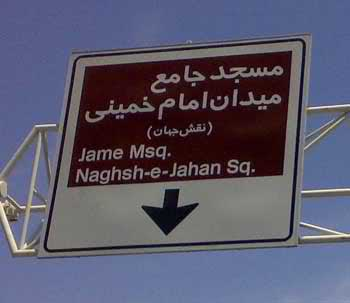
\includegraphics[height=4cm]{masjed.jpg}}
\hspace{3mm}
\frame{
\includegraphics[height=4cm]{sign.png}}
\caption{
راست: تابلوی راهنما\cite{masjedJame}. چپ: علامت راهنمایی و رانندگی\cite{signPic}. }
\label{sign-pic}
\end{figure}

از آن‌جا که عمده‌ی اطلاعات این تابلوها، توسط متن‌ آن‌ها منتقل می‌شود، تشخیص آن‌ها در تصویر به تنهایی کافی نیست و اطلاعات موجود در تابلو، که بخش عمده‌ی آن شامل متن است، باید استخراج شود. الگوریتم‌های موجود برای تشخیص متن، نیازمند یک ورودی مناسب و دربردارنده‌ی متن تقطیع‌شده از پس‌زمینه هستند. از این رو، تشخیص مکان دقیق متن در تابلوی راهنما و تقطیع آن، دارای اهمیت ویژه‌ای می‌باشد. از طرفی، برای پاسخ‌گوییِ به‌هنگام، نیاز است این عمل به صورت بی‌درنگ انجام شود.

تشخیص تابلوی راهنما در محیط شهری، خود به تنهایی چالش برانگیز است و علت آن، غیرقابل پیش‌بینی بودن پس‌زمینه در محیط‌های شهری و وجود اجسام مشابه از نظر شکل کلی یا رنگ در تصویر است که تقطیع به روش‌های معمول را دشوار می‌کند. تابلوهای فروشگاه‌ها، بدنه‌ی خودروهای بزرگ‌ ویژه‌ی حمل و نقل که حاوی متن باشد و بنرهای تبلیغاتی، از نمونه‌ی این شباهت‌ها هستند. از طرفی، نویز در تابلوهای راهنمای موجود در محیط‌های شهری شدیدتر است که از دلایل آن می‌توان به آلودگی بیشتر، وجود نورها و انعکاس‌های اضافی زیاد و متفاوت در ساعات مختلف روز، و وجود موانع و تغییرات ناخواسته در تصویر مانند شاخ و برگ درختان و یا سایه‌ی ساختمان‌های اطراف که ممکن است بخشی از تابلوی راهنما را در تصویر دست‌خوش تغییر کنند، اشاره نمود. چالش دیگر در این مساله آن است که با تصاویر ثابت و مشخصی در هر فریم سر و کار نداریم و هر فریم موجود در ویدیوی ثبت‌شده در شرایط واقعی، با لرزش‌ها و تغییرات هندسی ناشی از حرکت خودرو همراه است که در شرایط متفاوت و زاویه‌دید‌های متفاوت، اثر متفاوتی بر ظاهر تابلوی راهنما خواهند داشت.


پس از تشخیص تابلوی راهنما، باید مکان‌یابی دقیق متن در تابلو و آماده‌سازی آن برای استفاده‌ی آتی در الگوریتم‌های شناسایی انجام شود. دقت پایین تصویر ورودی در الگوریتم‌های \lr{OCR} زبان انگلیسی، که به شدت بر ویژگی‌های حروف انگلیسی وابسته‌اند، تاثیر چندانی نخواهد داشت، چرا که حروف از هم جدا هستند و به آسانی در مراحل قبل تقطیع می‌شوند، حال آن‌که در زبان فارسی این‌گونه نیست و تقطیع اجزای متن و تشخیص آن‌ها دشوارتر است. همچنین چندشکلی بودن برخی حروف فارسی، فرایندهای معمول مانند دسته‌بندی و یا پیدا کردن عمل‌گرهای خاص برای تشخیص متن را دشوار می‌کند. بنابراین، خروجی مناسب برای الگوریتم \lr{OCR} فارسی، باید از دقت بالاتری در تقطیع برخوردار باشد. تهیه‌ی این ورودی مناسب، مستلزم تقطیع دقیق تصویر متن‌ِ یافت‌شده در تابلو است. وجود نویز و خدشه‌های احتمالی موجود در متن تابلو، و نیز تغییرات ناشی از نور و شرایط محیطی، این تقطیع دقیق را دشوار می‌سازد. از طرفی مکان‌یابی متن موجود در الگوریتم‌های موجود برای زبان انگلیسی، به ویژه در پیاده‌سازی‌های بی‌درنگ، از خواص آن زبان استفاده می‌کنند و برای مکان‌یابی متن فارسی، در برخی موارد، دچار مشکل می‌شوند. 

برای ارزیابی این مساله در زبان فارسی و در محیط شهری، پایگاه داده‌ای وجود ندارد و تهیه‌ی داده‌های مورد نیاز و کافی از سطح شهر و در شرایط مختلف، چالش دیگری خواهدبود.
در این پژوهش، تابلوهای راهنما را در ویدیوهای ترافیکی شهری تشخیص داده‌ خواهد‌شد و مکان متن فارسی در آن مشخص خواهد‌شد. سپس مکان متن مورد نظر، به پیش‌زمینه و پس‌زمینه، تقطیع خواهدشد. 
فرض‌های مساله به این صورت است که تابلوهای راهنما با رنگ‌های پس‌زمینه و پیش‌زمینه‌ی مشخص و محدود وجود دارند و شامل متن انگلیسی، متن فارسی و علامت هستند. ابعاد این تابلوها نیز مشخص است و از چند گونه‌ی محدود تجاوز نمی‌کند. مکان و جهت قرارگیری تابلو نسبت به جاده مشخص است و در ارتفاع خاصی قرار می‌گیرد و هرگونه تغییر هندسی، ناشی از حرکتِ خود خودرو خواهد بود. داده‌ها شامل تصاویری هستند که در ساعات گوناگون شبانه‌روز تهیه شده‌اند. همچنین داده‌ها در بازه‌ی خاصی از سرعت حرکت خودرو تهیه شده‌اند و ابزار تصویر برداری، در نقطه‌ی خاصی از خودرو ثابت شده‌است. 


\section{کارهای مرتبط} 
تا به حال، حجم زیادی از کار بر روی تشخیص علایم راهنمایی و رانندگی ارایه شده‌است\cite{survey}. تا کنون، به صورت خاص ۳ کار متفاوت بر روی حل مساله‌ی ما ارایه شده‌است. البته نویسندگان \cite{gonzalez1} در \cite{gonzalez2} نیز روشی مشابه را برای تشخیص و شناسایی علایم و تابلوها در شب ارائه نموده‌اند.

 در \cite{adaptive} تصویر با توجه به رنگ‌های معمول استفاده‌شده در تابلوهای راهنما و متن‌ آن‌ها، تقطیع شده‌است و یک ماسک برای تصویر به‌دست‌ آمده‌است که در آن پیکسل‌هایی که احتمالا مربوط به تابلوی راهنما هستند مشخص شده‌اند و باقی پیکسل‌ها به عنوان پس زمینه در نظر گرفته‌‌شده‌اند. این کار، با آستانه‌‌ای‌سازی\LTRfootnote{ Thresholding} در فضای رنگ \lr{HSI} و سپس دسته‌بندی اشکال صورت گرفته‌است. استفاده از این فضای رنگ، این روش را نسبت به تغییرات نوری تا حدی مقاوم نموده‌است. پس از تقطیع با رنگ و اتصال اجزای متصل به‌ هم، نواحی به‌دست آمده برای یافتن مناطق مستطیل شکل جست‌وجو می‌شوند. این امر از طریق مقایسه‌ی اثر شعاعیِ \lr{FFT} \LTRfootnote{ Fast Fourier Transform} آن ناحیه با اثر شعاعی \lr{FFT} یک مستطیل ایده‌آل محقق می‌شود‎. این روش که جزییات آن در \cite{FFT} آورده‌ شده‌است، نسبت به تغییرات زاویه‌ی دید، چرخش، و اعوجاج ناشی از افکنش\LTRfootnote{ Perspective} دوربین، مقاوم است که در شکل \ref{fft-pic} آورده شده‌است. 
 \begin{figure}[t]
\centering
\frame{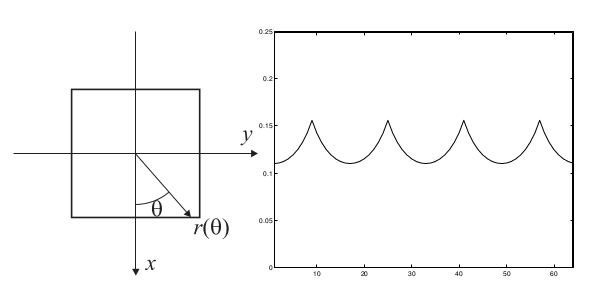
\includegraphics[height=4cm]{fft-pic.png}}
\caption{روش ارایه شده در \cite{adaptive}}
\label{fft-pic}
\end{figure}
 
 پس از آن، مستطیل‌های یافت‌شده با اعمال یک تبدیل هوموگرافی\LTRfootnote{ homography} که با توجه به بیشینه‌های موجود در اثر شعاعی محاسبه‌شده که به چهارگوشه‌ی مستطیل تعلق دارند، به دست می‌آید،  در جهت و راستای درست قرار داده‌می‌شوند.  در نهایت با تحلیل هیستوگرام رنگ و روشنایی، تقطیع نواحی تابلوی راهنما به پس‌زمینه و پیش‌زمینه انجام شده‌است. این روش در برابر تبدیلات هندسی مقاوم است، اما در برابر تغییر رنگ ضعیف است. همچنین این روش به صورت بی‌درنگ نیست و پردازش‌ها بر روی تصاویر گرفته‌شده‌ی مناسب انجام شده‌اند و هیچ‌گونه تحلیل یا نتیجه‌ی تجربی از سرعت اجرای الگوریتم ارایه نشده‌است.

در \cite{fromVid}، نواحی هم‌رنگ توسط الگوریتم \lr{k-means} استخراج می‌شوند و نواحی مسطح عمود بر محور دوربین انتخاب می‌شوند. برای این کار از سه یا چند نقطه‌ی هر ناحیه در دو فریم‌ متوالی استفاده شده‌است و به همین دلیل، این روش نیازمند دنبال کردن نقاط متناظر در دو یا چند فریم با دقت بالا می‌باشد. در این روش از ویژگی‌های گوشه، تحلیل رنگ، هم‌ترازی هندسی و مدل‌های ترکیبی گاسی استفاده شده‌است و به تشخیص متن با دقت ۸۹\% رسیده‌است، اما تحلیلی از دقت تشخیص تابلوهای راهنما و یا تشخیص مکان متن در اختیار گذاشته‌ نشده‌است و از طرفی، داده‌های آزمایش در دسترس عموم قرار نگرفته‌است و مقایسه‌ای به‌دست نمی‌دهد. همچنین در این روش، پس از ادغام فریم‌های متوالی، مکان متنِ یافت‌شده مشخص می‌شود و برای \lr{OCR‌} به مرحله‌ی بعدی می‌رود، و در هر فریم مکان متن موجود از دقت پایینی برخوردار است. شمای این روش در شکل \ref{vid-pic} آورده شده‌است. 
\begin{figure}[t]
\centering
\frame{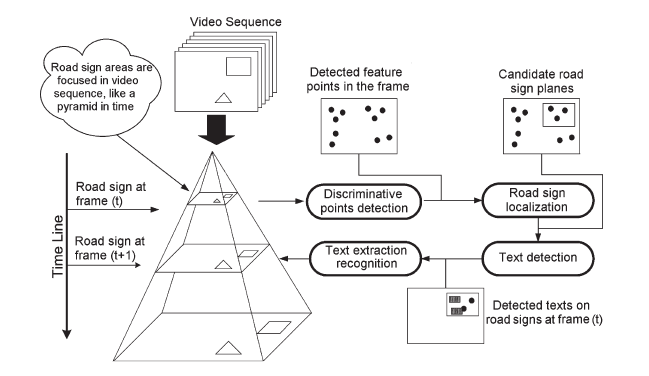
\includegraphics[width=13cm]{video.png}}
\caption{روش ارایه شده در \cite{fromVid}}
\label{vid-pic}
\end{figure}

در \cite{gonzalez1} ، از یک مدل \lr{BOVW}\LTRfootnote{ Bag of Visual Words} برای تشخیص تابلوی راهنما استفاده شده‌است که بر خلاف روش‌های موجود که از ویژگی‌های هندسی یا گوشه‌ها استفاده می‌کنند، از توصیف‌گرهای محلی به‌دست آمده از نقاط مهم تصویر استفاده می‌کند. این نقاط مهم، در یک فاز تقطیع مبتنی بر رنگ به‌دست می‌آیند. ایده‌ی استفاده از مدل \lr{BOVW} از تحلیل اسناد گرفته شده‌است که در آن یک سند با فرکانس تکرار کلماتش، بدون توجه به ترتیب قرارگیری کلمات، توصیف می‌شود و از این فرکانس‌ها برای دسته‌بندی اسناد استفاده می‌شود. در ارایه‌ی تصویر با این مدل نیز از همین ایده استفاده شده‌است، با این تفاوت که ویژگی‌های محلی نقش کلمات را بازی می‌کنند. ویژگی‌های محلی \lr{SIFT}، \lr{C-SIFT}، \lr{Hue Histogram}، \lr{Hue-SIFT}، \lr{RGB-SIF} و  \lr{TCH}\cite{tch} به عنوان توصیف‌گر محلی بررسی شده‌اند. دسته‌بندی نواحی با استفاده از \lr{SVM} و \lr{Naïve Bayes} بررسی شده‌اند. به دلیل کند بودن \lr{SVM}، از \lr{Naïve Bayes} استفاده شده‌است. البته نرخ تشخیص‌های اشتباه آن از \lr{SVM} بیشتر بوده‌است و به خاطر سرعت بیشتر ترجیح داده‌شده‌است. همگرایی دسته‌بندی تنها به ازای توصیف‌گرهای محلی \lr{SIFT، \lr{Hue} Histogram} و \lr{TCH} حاصل شده‌است که مقایسه‌ای از این سه توصیف‌گر نیز ارایه شده‌است، هرچند علت عدم‌ هم‌گرایی در استفاده از دیگر ویژگی‌ها بررسی نشده‌است. این روش در جاده‌های بین‌شهری جواب بسیار مناسبی دارد ولی در نواحی شهری از دقت خوبی برخوردار نیست.
شمای کلی این روش در شکل \ref{gonzalez1-pic} آمده است. 
\begin{center}
\begin{figure}[h]
\centering
\frame{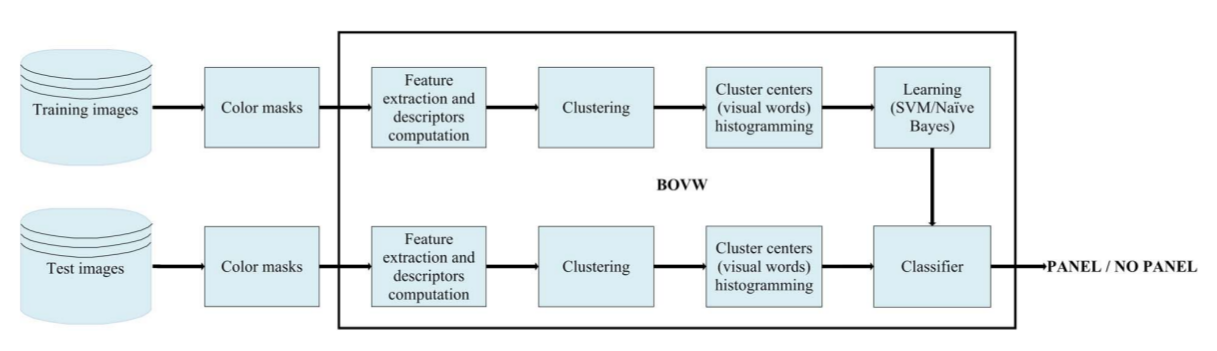
\includegraphics[width=13cm]{pic1.png}}
\caption{روش ارایه شده در \cite{gonzalez1}}
\label{gonzalez1-pic}
\end{figure}
\end{center}
روش‌های ترکیبی در مکان‌یابی متن بازدهی و عملکرد خوبی در محیط‌های شلوغ داشته‌اند، مانند \cite{hybrid} که از ترکیب یک روش \lr{CC-Based}  و یک روش مبتنی بر یادگیری \lr{P-N} که با یک \lr{SVM} پیاده‌سازی شده‌است، استفاده‌ کرده‌است؛ هرچند در فاز یادگیری ماشین کند عمل می‌کند. دسته‌ی دیگری از روش‌های موثر، روش‌های مبتنی بر گروه‌بندی بر اساس ویژگی‌های هندسی و ظاهری هستند\cite{group}. نمونه‌ی استفاده‌ی این دو روش برای متن فارسی در ‎\cite{faVid} و \cite{faAut} آمده‌است. در این میان، \cite{faVid} تنها بر روی ویدیوهای تلویزیونی پاسخ‌گو است و  در \cite{faAut} نیز پردازش بر روی تصویر انجام گرفته‌‌ شده‌است و تحلیلی از کارایی ارایه نشده‌است. همچنین این روش نسبت به تغییرات رنگ مقاوم نیست و در روشی که از لبه‌ها نیز استفاده شده‌است، دقت خوبی ارایه نشده است. 
\section{روش‌ انجام پژوهش}

در مرحله‌ی اول، باید در هر فریمِ مورد پردازش، وجود یا عدم وجود تابلوی راهنما را دریابیم و در صورت وجود، مکان قطعه‌ی مربوط به تابلوی راهنما را مشخص کنیم. تشخیص آن‌که در فریم موجود، تابلوی راهنما وجود دارد یا خیر، خود امری مهم است، چرا که سبب می‌شود از پردازش‌های اضافی آتی جلوگیری کنیم. همچنین در صورت وجود تابلوی راهنما در تصویر، جست‌وجوی متن را تنها در آن ناحیه انجام خواهیم داد که خود سبب افزایش کارایی خواهد بود. 

برای استفاده از روش‌های موجود، از جمله \cite{gonzalez1}، مسایل مهمی برای بررسی و در صورت نیاز، بهبود آن وجود دارد. برای مثال استفاده‌ی موفق از \lr{C-SIFT}، که بر خلاف \lr{SIFT}، در فضای رنگی عمل می‌کند، می‌تواند فاز تقطیع رنگی را حذف کند. یافتن ویژگی مناسبی مانند \lr{C-SIFT} یا ویژگی‌های دیگر، برای استفاده در مدل \lr{BOVW} که در \cite{gonzalez1} آمده‌است نیز می‌تواند مورد بررسی قرار گیرد و یا از مدل بهتری برای توصیف تصویر استفاده‌کرد. از دیگر موارد مهم برای بررسی، نحوه‌ی پیدا کردن نقاط مهم است که می‌توان از مدل‌های برجسته‌تر و به‌روزتر، مانند مدل‌های توجه مبتنی بر بینایی \cite{attention} یا دیگر روش‌های استفاده‌شده در کارهای موجود در زمینه‌ی تشخیص علایم راهنمایی و رانندگی \cite{survey} استفاده نمود. همچنین باید بررسی دقیق‌تری بر نحوه‌ی عملکرد انواع الگوریتم‌های دسته‌بندی برای این مساله‌ی خاص صورت گیرد تا در صورت نیاز جای‌گزین روش انتخاب‌شده در \cite{gonzalez1}، یعنی \lr{Naïve Bayse} نمود. برای نمونه از \lr{SVM} نیز برای دسته‌بندی در این مساله استفاده شده‌است اما با مدل \lr{BOVW} و با استفاده از ویژگی‌های یاد‌شده در \cite{gonzalez1}، دقت مطلوب را نداشته‌است. علاوه بر مدل \lr{BOVW}، مدل‌های دیگری از بازنمایی مساله و توصیف تابلو نیز قابل بررسی هستند، که از جمله‌ی آن‌ها مقایسه‌ی اثر شعاعی تبدیل فوریه است که در بخش سوابق علمی بررسی کرده‌ایم. به‌کار بردن تبدیل هاف، نماینده‌ی دیگری برای حل این بخش از مساله خواهد بود. 


در مرحله‌ی دوم، برای تشخیص و مکان‌یابی متن فارسی در تابلوی راهنما، و تقطیع آن به پیش‌زمینه و پس‌زمینه، چالش‌هایی همچون پیوستگی حروف در متن فارسی و چندشکل داشتن برخی از حروف وجود دارد. این سبب می‌شود که ترکیبات حروف، به اشکال پیچیده‌تری نسبت به ترکیبات حروف انگلیسی منجر ‌شود و در نتیجه، عمل دسته‌بندی را دشوارتر می‌کند. خود عمل تشخیص و مکان‌یابی متن در تصویر نیز با چالش‌هایی روبه‌رو است که در صورت شلوغ بودن پس‌زمینه کار را دشوار می‌کند. در تابلوهای راهنما این موضوع مطرح نیست اما با مراجعه به کارهایی که برای این گونه تشخیص‌ها انجام شده‌اند، از جمله \cite{hybrid} و \cite{group}، می‌توان دقت تشخیص در پس‌زمینه‌های خلوت مانند تابلوهای راهنما‌ را بالا برد. این روش‌ها معمولا به دو دسته‌ی \lr{CC-Based}  که مبتنی بر اجزای متصل است، و روش‌های مبتنی بر ناحیه، تقسیم می‌شوند. این دو رویکرد را می‌توان به ترتیب پایین‌به‌بالا و بالابه‌پایین در نظر گرفت. در روش‌های مبتنی بر اجزای متصل، از ویژگی‌های معمول متن، مانند هم‌رنگ بودن اجزا، اندازه‌ی یکسان، هم‌ترازی هندسی و غیره استفاده می‌شود. در حالی که در روش‌های مبتنی بر ناحیه، از روش‌های یادگیری برای تقسیم تصویر به نواحی متن و غیر متن استفاده‌می‌شود. حل مساله با انتخاب یکی از این دو روش و یا یک روش ترکیبی (روش دسته‌بندی ناحیه و روش تشخیص اجزای متصل)، و استفاده از خواص زبان فارسی که در \cite{faVid} و \cite{faAut} آمده‌اند، قابل حل خواهد بود. روش‌های مبتنی بر گروه‌بندی بر اساس ویژگی‌های هندسی و ظاهری، نماینده‌ی دیگری برای حل این بخش از مساله خواهند بود.

\newpage
%دستوری برای به حالت عادی درآمدن اندازه فونت‌ها 
\small
%ایجاد «مراجع»
\begin{thebibliography}{99}

\begin{LTRitems}

\resetlatinfont

\bibitem{benz}
Dickmanns, Ernst D., and Alfred Zapp. "Autonomous high speed road vehicle guidance by computer vision." {\em In International Federation of Automatic Control. World Congress (10th). Automatic control: world congress.}, vol. 1. 1988.

\bibitem{gonzalez1}
González, Álvaro, Luis M. Bergasa, and J. Javier Yebes. "Text detection and recognition on traffic panels from street-level imagery using visual appearance." {\em Intelligent Transportation Systems, IEEE Transactions on.}, vol 15, no. 1 (2014): 228-238.

\bibitem{masjedJame}
Jame Msq. Naghsh-e-Jahan Sq. Traffic Panel photograph, viewed 23 April 2014,
<http://oi1.tinypic.com/68ktoq9.jpg>.

\bibitem{signPic}
Entrance Forbidden, Traffic Sign photograph, viewed 23 April 2014,
<http://upload.wikimedia.org/wikipedia/commons/thumb/e/ee/Zeichen\_267.svg/270px-Zeichen\_267.svg.png>.

\bibitem{survey}
Mogelmose, Andreas, Mohan M. Trivedi, and Thomas B. Moeslund. "Vision-based traffic sign detection and analysis for intelligent driver assistance systems: Perspectives and survey." {\em Intelligent Transportation Systems, IEEE Transactions on.}, vol 13, no. 4 (2012): 1484-1497.

\bibitem{gonzalez2}
González, Álvaro, Miguel Angel Garrido, David Fernández Llorca, Miguel Gavilán, J. Pablo Fernández, Pablo F. Alcantarilla, Ignacio Parra. "Automatic Traffic Signs and Panels Inspection System Using Computer Vision." {\em Intelligent Transportation Systems, IEEE Transactions on,}. vol 12, no. 2 (2011): 485-499.

\bibitem{adaptive}
Reina, A. Vázquez, RJ López Sastre, S. Lafuente Arroyo, and P. Gil Jiménez. "Adaptive traffic road sign panels text extraction." {\em In Proceedings of the 5th WSEAS International Conference on Signal Processing, Robotics and Automation,} pp. 295-300. World Scientific and Engineering Academy and Society (WSEAS), 2006.

\bibitem{FFT}
Gil-Jimenez, P., S. Lafuente-Arroyo, H. Gomez-Moreno, F. Lopez-Ferreras, and S. Maldonado-Bascon. "Traffic sign shape classification evaluation. Part II. FFT applied to the signature of blobs." {\em In Intelligent Vehicles Symposium, 2005. Proceedings. IEEE,} pp. 607-612. IEEE, 2005.

\bibitem{fromVid}
Wu, Wen, Xilin Chen, and Lei Yang. "Detection of text on road signs from video." {\em Intelligent Transportation Systems, IEEE Transactions on,}. vol 6, no. 4 (2005): 378-390.

\bibitem{tch}
Van De Sande, Koen EA, Theo Gevers, and Cees GM Snoek. "Evaluating color descriptors for object and scene recognition." {\em Pattern Analysis and Machine Intelligence, IEEE Transactions on,}. vol 32, no. 9 (2010): 1582-1596.

\bibitem{hybrid}
Pan, Yi-Feng, Xinwen Hou, and Cheng-Lin Liu. "A hybrid approach to detect and localize texts in natural scene images." {\em Image Processing, IEEE Transactions on,}. vol 20, no. 3 (2011): 800-813. 

\bibitem{group}
Yi, Chucai, and YingLi Tian. "Text string detection from natural scenes by structure-based partition and grouping." {\em Image Processing, IEEE Transactions on,}. vol 20, no. 9 (2011): 2594-2605.

\bibitem{faVid}
Moradi, Mohieddin, and Saeed Mozaffari. "Hybrid approach for Farsi/Arabic text detection and localisation in video frames." {\em IET Image Processing,}. vol 7, no. 2 (2013): 154-164.

\bibitem{faAut}
Darab, Maryam, and Mohammad Rahmati. "A Hybrid Approach to Localize Farsi Text in Natural Scene Images." {\em Procedia Computer Science 13,}. (2012): 171-184.

\bibitem{attention}
Kastner, Robert, Thomas Michalke, Thomas Burbach, Jannik Fritsch, and Christian Goerick. "Attention-based traffic sign recognition with an array of weak classifiers." {\em In Intelligent Vehicles Symposium (IV),}. 2010 IEEE, pp. 333-339. IEEE, 2010.

\end{LTRitems}

\end{thebibliography}

\end{document} 
